\chapter{Evaluation}

The evaluation is conducted on several independent scenarios. As mentioned in chapter 1 the thesis relies on four subtasks that need to be solved. First, the forwarding should rely on MAC addresses of the WiFi network interface (also called net devices) and not on the different faces. The second subtask is to implement a forwarding strategy that can be used with the MAC addresses. The third part is to add mobility to the intermediate nodes while the fourth part is to improve the forwarding strategy. Every scenario is evaluated and compared to the ndnSIM's multicast strategy \texttt{nfd::fw::MulticastStrategy}, which has been implemented in ndnSIM version 2.0 as basic multicast strategy. The thesis will refer to this multicast strategy as the base strategy or only base. It basically receives an interest and forwards it to all available faces of the node except the receiving one. The newly implemented forwarding strategy will often be referred to as the new strategy or the improved strategy.

To achieve comparability the scenario and trace-files are copied into a clean base installation of ndnSIM version 2.0. All parameters are kept equal. Then it is run once on the clean installation and once on the improved one. In the first scenario, the implementation of the MAC addresses and the forwarding mechanism is tested and evaluated. In the second scenario, mobility is introduced with changes to the strategy. The different scenarios are tested for Interest/Data ratio, latency, congestion and number of distinct routes, although distinct routes do not exist in the already existent multicast strategy. It is introduced as part of the thesis for the new implementation.

\section{Evaluation Environment}

All tests are run on the ns-3 network simulator with ndnSIM version 2.0.  As WiFi standard 802.11a was used, which means each node has a transmission range of approximately 120 meters in open space \cite{wifi80211a} . For the propagation delay \texttt{ns3::Constant}\texttt{SpeedPropagation}\texttt{DelayModel} was used and for the propagation loss \texttt{ns3::Three}\texttt{LogDistance}\texttt{Propagation}\texttt{LossModel} and \texttt{ns3::}\texttt{Nakami}\texttt{Propagation}\texttt{LossModel} were used. Interest lifetime is set to 4 seconds and the retransmission timeout to 500ms. Data packet size is 1200kb.

\subsection{Topology and Mobility}

The topology of the nodes and their movement is a fundamental factor that should be considered carefully. In order to be able to run specific tests, the nodes need to be spaced accordingly. Since WiFi 802.11a is used in this theses the nodes should not exceed 200 meters or the connection will be lost. On the other hand putting them to near together will introduce problems in collisions, retransmissions and lost packets. The nodes will not be able to handle flooding efficiently when clustered all together. Random movement is another problem that can lead to unwanted problems and lost routes.
 
The topology is created within a trace file that can be read by the \texttt{Ns2MobilityHelper} helper class and is fully supported by the ns-3 network simulator. The initial positions of the nodes within the cartesian coordinate system are placed inside the file by specifying the node, it's x-value and it's y-value as shown in figure \ref{fig:ns2traceFileStatic}:

\begin{figure}[H]
  \centering
  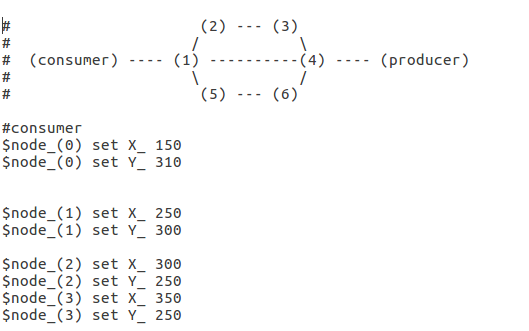
\includegraphics[scale=0.6]{chapter-5/ns2traceFileStatic}
  \caption{Node positioning in NS2 trace files}
  \label{fig:ns2traceFileStatic}
\end{figure}

\clearpage

This scenario has been used for the static 8 node simulations. For the dynamic scenario, movement had to be added through special statements in the trace file. Every statement specifies the time at which the movement will take place, the node which has to be moved, the new destination and speed. The node will stop when it arrives at the new destination or when a new statement changes its course and speed. Figure \ref{fig:ns2traceFileDynamic} shows few lines from the trace file used in the dynamic 16 node scenario.

\begin{figure}[H]
  \centering
  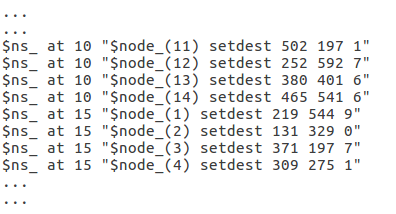
\includegraphics[scale=0.6]{chapter-5/ns2traceFileDynamic}
  \caption{Node movement in NS2 trace files}
  \label{fig:ns2traceFileDynamic}
\end{figure}

\clearpage

\section{Results for a Static 8 Nodes Scenario}

The first scenario is a static 8 node scenario with one consumer on the left and one producer on the right. 6 intermediate nodes are placed in between as seen in figure \ref{fig:scenario1}. Every node has 3 net devices with distinct MAC addresses. They allow on one hand to send and receive simultaneously, while extending on the multi-path idea. The paths are determined by the FIB entries that have been configured with MAC addresses from data being forwarded downstream. Therefore the first segment of an Interest can be requested through the first net device. The second segment is requested through the second net device and the third segment through the third net device. The fourth segment would be sent again through the first net device. That is achieved by a static counter and a modulo operation leading to different routes.

\vspace{5mm} %5mm vertical space

\begin{figure}[H]
  \centering
  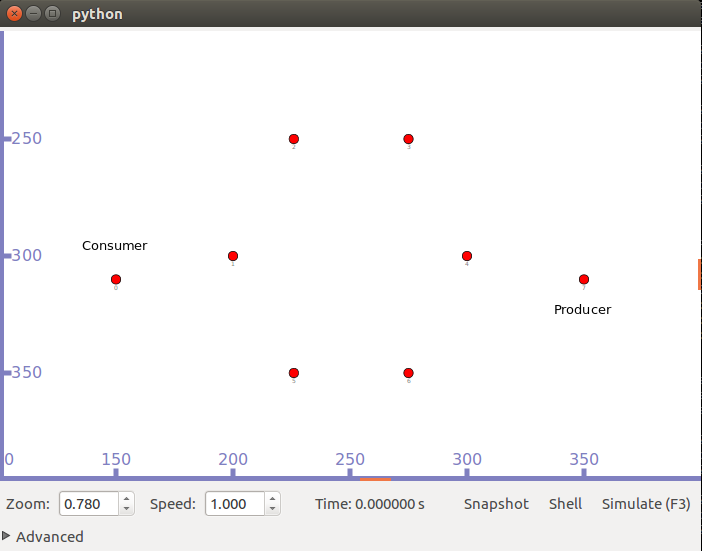
\includegraphics[scale=0.5]{chapter-5/scenario1}
  \caption{Basic static scenario with 8 nodes, 1 consumer and 1 producer}
  \label{fig:scenario1}
\end{figure}

\vspace{5mm} %5mm vertical space

The runs have been conducted for 100, 200, 300 and 600 seconds each. The consumer was configured to sent out Interests at a frequency of 3 Interests per second. For the ratio, received Data over send Interests only distinct packets were counted. Retransmissions were ignored. The average latency was measured in nanoseconds, as the time difference of the Interest leaving the consumer and the corresponding Data packet being received at the consumer added together and divided by all successful Interest requests.

\vspace{5mm} %5mm vertical space

\begin{figure}[H]
  \centering
  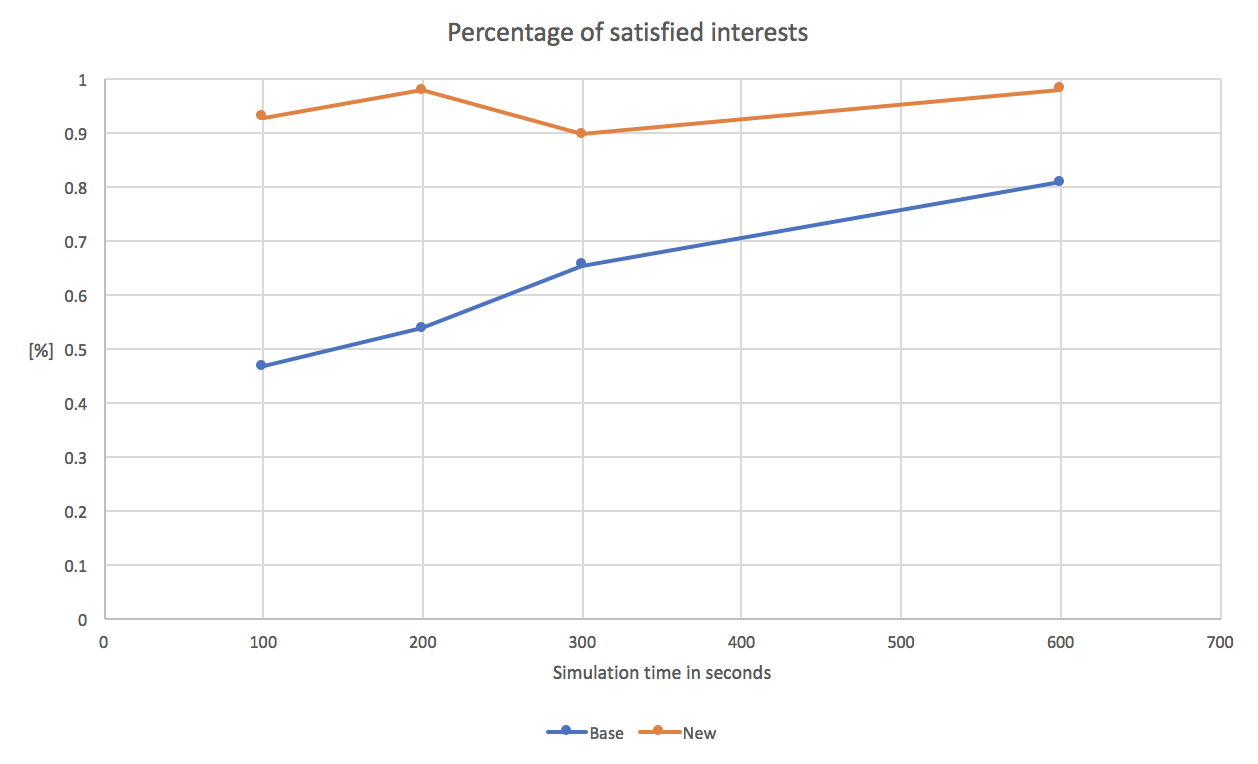
\includegraphics[scale=0.6]{chapter-5/staticS1ratio}
  \caption{Satisfaction ratio at different simulation times for both implementations}
  \label{fig:staticS1ratio}
\end{figure}

\vspace{5mm} %5mm vertical space

Figure \ref{fig:staticS1ratio} compares the ratio of satisfied Interests (Interests send / Data received back) over simulation time. A better ratio has been observed for the new implementation at all simulation times. The difference is biggest at a run time of 100 seconds. At a run time of 600 seconds, the difference has been reduced to 0.171. That is due to the amount of Interests and Data being in transition. As the number of satisfied Interest messages constantly rises over time, the unsatisfied Interest will not keep getting more since retransmissions will be made after new Interests are introduced to the network.

Figure \ref{fig:staticS1iod} shows that the ratio of satisfied Interests over simulation time alone (as shown in Figure \ref{fig:staticS1ratio}) does not make any statement about a number of the Interests sent towards a potential content producer and the amount of received Data. With the base implementation, there is not much gain with increased simulation time whereas with the new implementation the gain nearly doubles. The reason for that observation is explained with congestion. Broadcasting the Interest at each node leads to an exponential increase in the packets being retransmitted within the network leading to congestion, loss of packets and retransmissions. The new implementation floods the network only with the first Interest and uses configured routes for all further Interests leading to much less traffic. Retransmissions have been observed at the consumer and although the new implementation has fewer retransmissions (around 15 percent) it is not very significant and they happen on a much higher transmission rate. It can be expected that the retransmission rate is strongly correlated with the retransmission timer in the consumer and the lifetime of the Interest itself.

\clearpage

\begin{figure}[H]
  \centering
  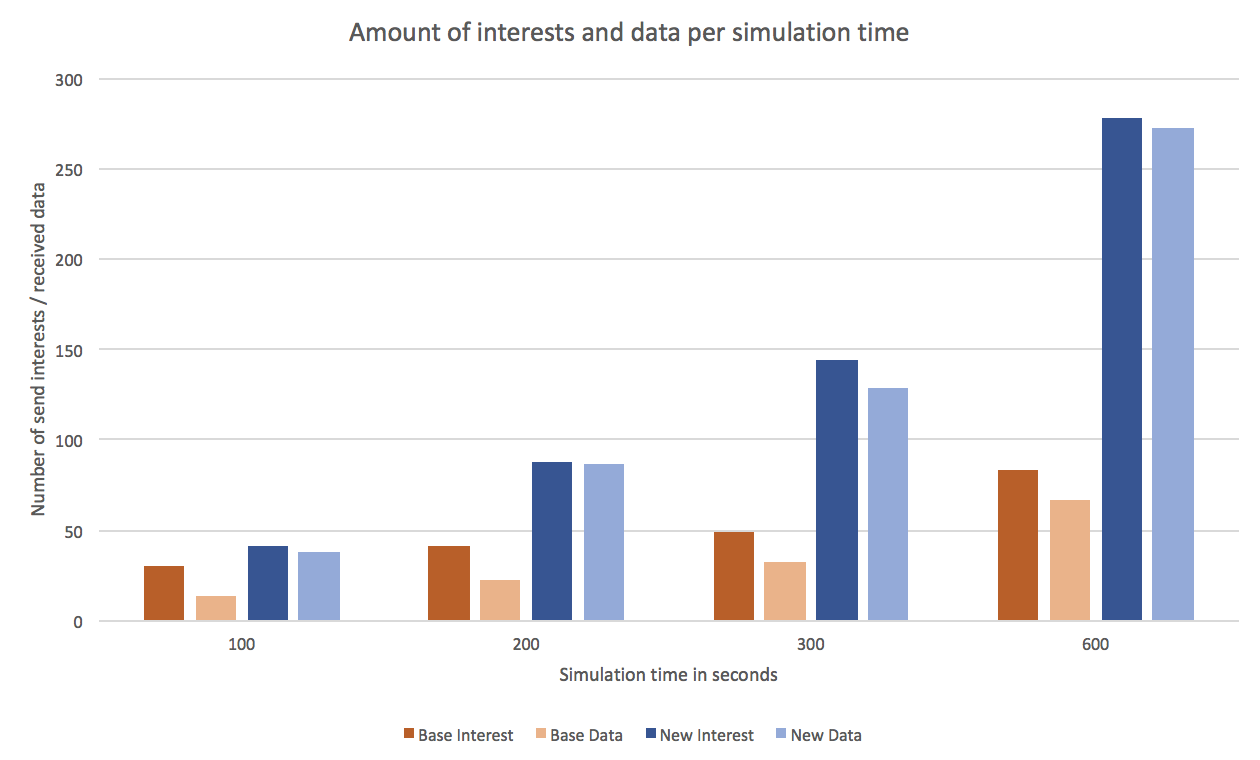
\includegraphics[scale=0.6]{chapter-5/staticS1iod}
  \caption{Number of sent and received packets over simulation time}
  \label{fig:staticS1iod}
\end{figure}

Figure \ref{fig:staticS1latency} shows how the latency changes with the simulation time and chosen implementation. As expected from \ref{fig:staticS1iod} the latency increases significantly with congestion and retransmissions in the base implementation of the multicast strategy. During the first 100 seconds, the latency reaches 40 seconds. At the end of the simulation it is about 140 seconds. The new implementation has a much lower latency, starting with around 11 seconds for the first 100 seconds of the simulation. Then it increases slightly till around 15 seconds for 600 seconds of simulation. This also shows that congestion and retransmission stay relatively constant for the new implementation.

\clearpage

\begin{figure}[H]
  \centering
  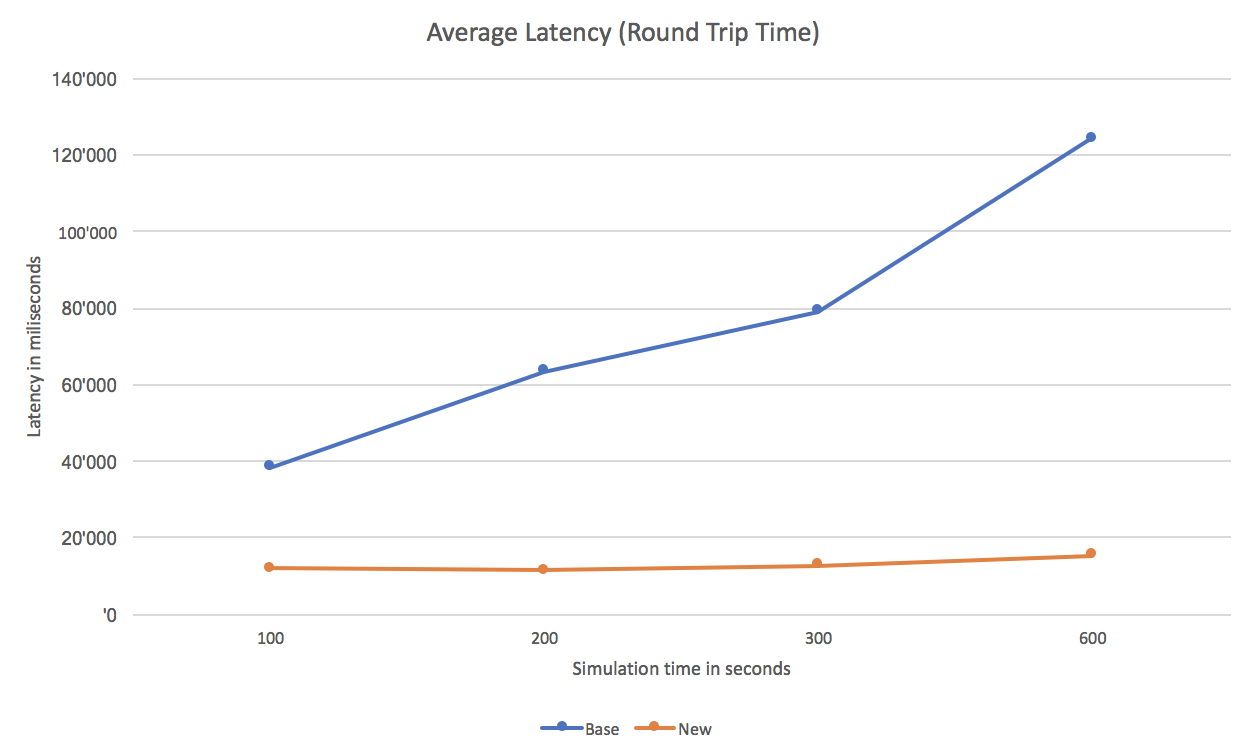
\includegraphics[scale=0.6]{chapter-5/staticS1latency}
  \caption{Latency of both implementations over simulation time}
  \label{fig:staticS1latency}
\end{figure}

The implementation has been tested with overhearing of data coming back and adding the route to the FIB entries but with a higher cost. If the Data packet was intended for the receiving node, the node added or updated the FIB with the new information and attached cost 111 to this specific next hop. The number 111 was randomly chosen and represents a relative low cost. If the Data was only overheard (unsolicited) a FIB entry was updated or created with cost 222 instead of ignored and dropped immediately to save resources. The results were slightly worse than the above proposed implementation, but still much better than the base one.

\vspace{5mm} %5mm vertical space

Since one to three new FIB entries were added to every node, an additional approach was to test, if instead of broadcasting or forwarding the Interest to only one next hop, better results could be achieved by forwarding the Interest to two or three distinct next hops. This yielded again worse results and led to the above proposed implementation.

\vspace{5mm} %5mm vertical space

Having more than one valid next hop within a FIB entry did not result in more routes taken by the Interests. Instead of alternating between possible next hops only the first one (with the lowest cost) was chosen and the Interest forwarded to. Incrementing each next hop's cost by one after forwarding through it and sorting the FIB's next hops did increase the number of different routes effectively used. The next hops within the FIB entry were selected in alternating fashion. Unfortunately, that did not improve the overall performance. It decreased it despite having more routes to chose from. The reason for this behavior is how ndnSIM translates FIB next hop's cost into transmission time. The lower the cost the more reliable and faster the Interest is forwarded. For example re-setting the cost to 50 after reaching 150 while incrementing all forwarded FIB next hops led to significantly better results. If in contrast, the cost was initially set to 250 and reset to this value after reaching 350, the overall performance was significantly worse. Since that is true for both scenarios equally, has not been further investigated.

\section{Results for a Dynamic 16 Nodes Scenario}

For the dynamic scenario, 8 further nodes were introduced. All 14 intermediate nodes have been randomly scattered between the consumer and the producer. Random movement was added to the trace file by changing direction and speed of every intermediate node at 5 second intervals. This random movement has been achieved by a self written script, that generates random numbers within the grid range (between 100 and 600) for the new x and y coordinates and random numbers between 0 and 10 for the speed. The values were inserted into the correct statements as shown in \ref{fig:ns2traceFileDynamic}. The net devices remain to be three. Retransmission time is set to 500 milliseconds, while the Interest lifetime also remains at 4 seconds. 

Figure \ref{fig:scenario2} shows the topology at the beginning of the simulation. The consumer and producer are marked in the figure and remain static. Only intermediate nodes move in a random manner at different speeds. The distance between consumer and producer as been increased to about 450 meters.

\vspace{5mm} %5mm vertical space

\begin{figure}[H]
  \centering
  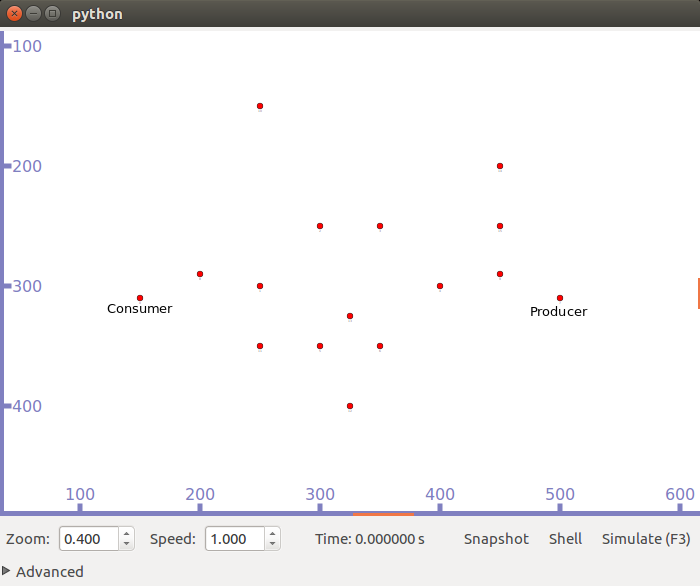
\includegraphics[scale=0.4]{chapter-5/scenario2}
  \caption{Ad-hoc scenario with 16 nodes and movement, 1 consumer and 1 producer}
  \label{fig:scenario2}
\end{figure}

\vspace{5mm} %5mm vertical space

For the static scenario, it was sufficient to keep the configured routes constant, since no movement changed the topology. In this scenario, though, by moving intermediate nodes, the strategy may possibly lead to loosing the connection altogether (if the nodes move too far away). The base implementation of ndnSIM does not have this problem since it has no specific routes to follow and basically broadcasts the Interest all over again using the next best node available. The trace file was randomly generated in order to give a realistic scenario and the above problem can be seen around simulation time: 200 seconds in Figure \ref{fig:scenario2extended}. This problem is also noticed in the numeric data.

\vspace{5mm} %5mm vertical space

\begin{figure}[H]
  \centering
  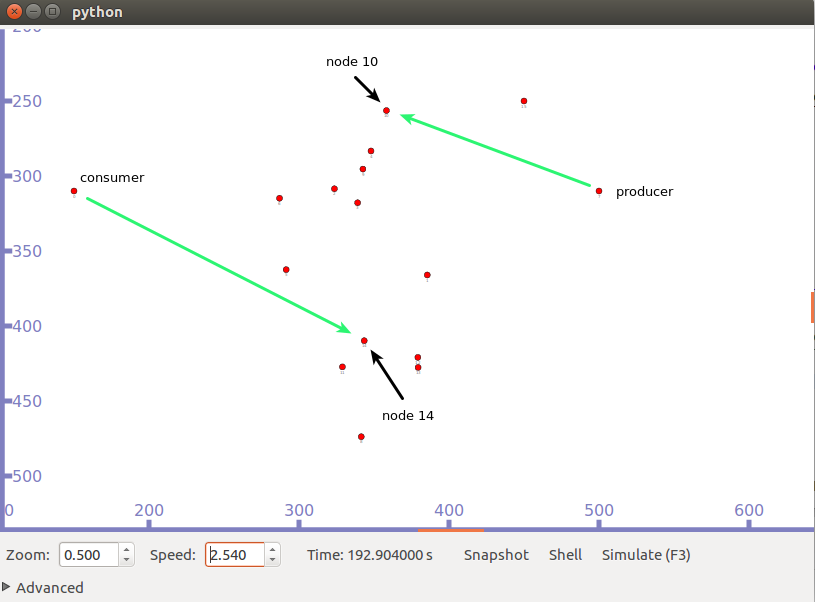
\includegraphics[scale=0.4]{chapter-5/scenario2extended}
  \caption{Node 10 is one of the producer preferred nodes while node 14 is one of the consumer preferred nodes}
  \label{fig:scenario2extended}
\end{figure}

To address the aforementioned problem, the Interest is forwarded to three FIB next hops (instead of only one) and making the strategy multicast to three nodes upstream the default. Sending the Interest to three MAC addresses increases robustness at the cost of generating more traffic, but overall leading to much better results without congesting the network.

Figure \ref{fig:scenario2ratio} shows the ratio of sent Interest packets over satisfied ones. The new implementation starts from 71.8\% satisfaction rate for the first 100 seconds of simulation and goes up to almost 90\% for the 600 seconds simulation. The ndnSIM base implementation starts lower, but as time passes by, the Interests get satisfied through broadcasting and the satisfaction rate rises up to 74.3\%.

\begin{figure}[H]
  \centering
  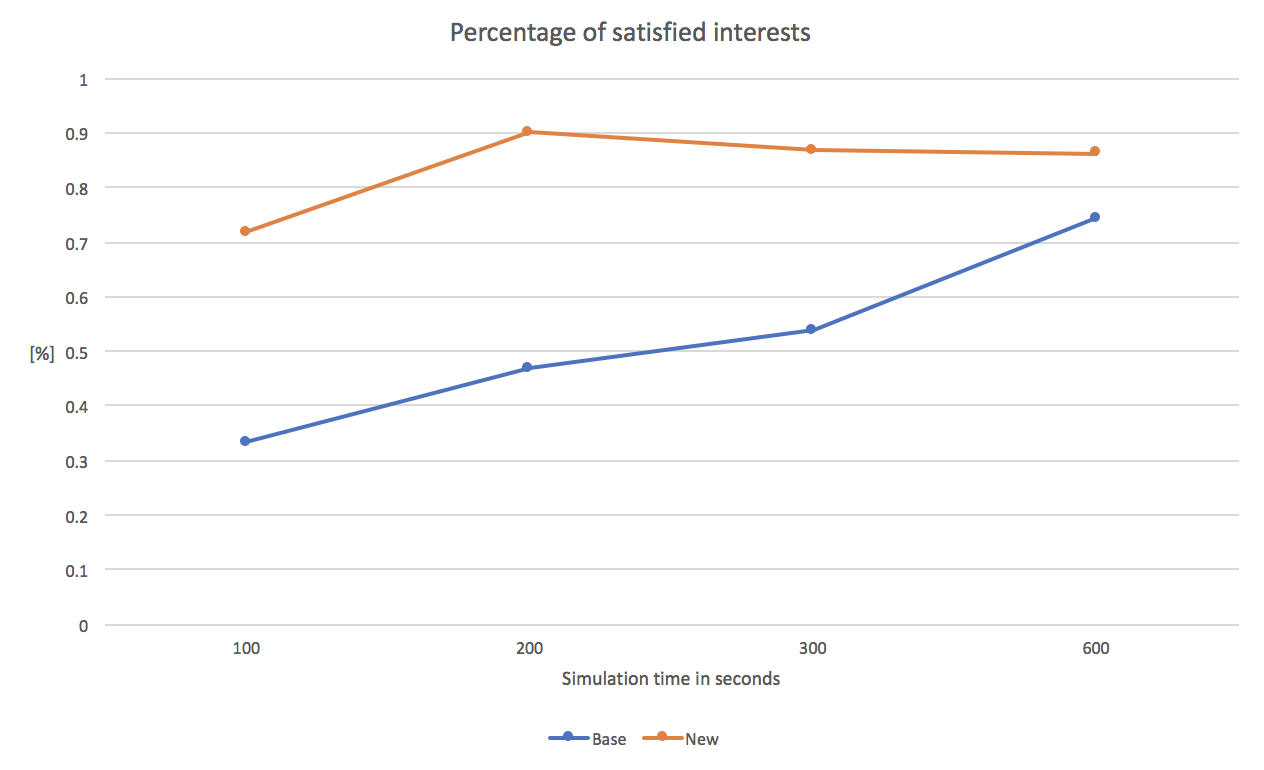
\includegraphics[scale=0.6]{chapter-5/scenario2ratio}
  \caption{Satisfaction ratio at different simulation times for both implementations with mobility}
  \label{fig:scenario2ratio}
\end{figure}

\vspace{5mm} %5mm vertical space

Like in the static scenario it is important to look at the overall throughput and set the satisfaction ratio into context of send and satisfied Interests. Figure \ref{fig:scenario2iod} shows the base implementation in brown colour. The dark bar shows the Interests send upstream towards a potential content producer, while the lighter bar shows the satisfied Interests. The ratio obtained in \ref{fig:scenario2ratio} is seen once again by comparing the bars of one color per simulation time to each other. The new implementation has not only a better ratio of satisfied Interests over simulation time, but also is able to send and receive more data. The reason is that the nodes are targeted specifically by the MAC address and do not congest the network even if send to three upstream addresses.
The new implementation sends 39 Interests out and receives 28 Data that satisfy the Interests in the first 100 seconds of the simulation. The next 100 seconds roughly doubles the Interests being sent and satisfied, whereas the next 100 seconds result in a decrease of newly satisfied Interests. That problem was described above and can be seen figure \ref{fig:scenario2extended}. Different trace-files led to different results and whenever a clustering of the intermediate nodes was observed the successfully sent out and satisfied Interests also slowed down. The clustering issue is also a problem for the ndnSIM base implementation strategy, but preferred nodes by FIB entries only pose a problem to the new implementation that needs further attention.

\clearpage

\begin{figure}[H]
  \centering
  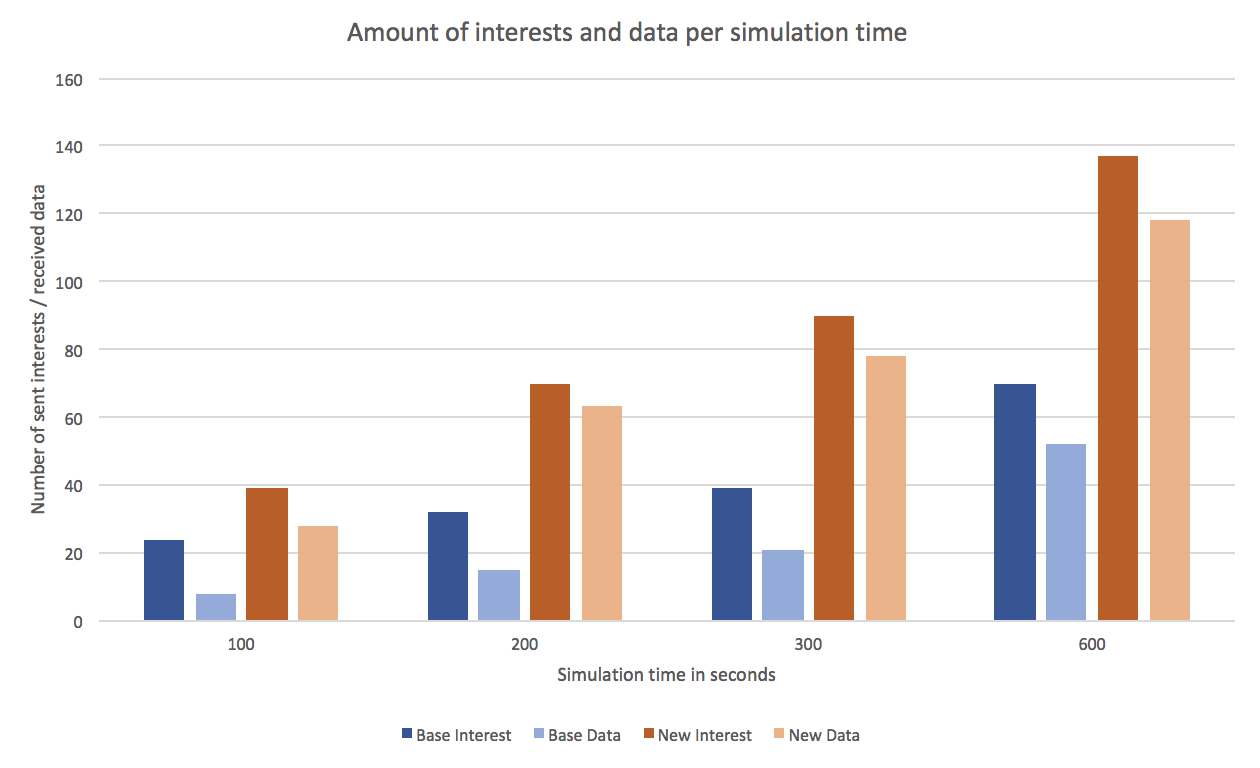
\includegraphics[scale=0.6]{chapter-5/scenario2iod}
  \caption{Number of sent and received packets over simulation time}
  \label{fig:scenario2iod}
\end{figure}

\vspace{5mm} %5mm vertical space

Figure \ref{fig:scenario2latency} shows the observed latency for both implementations. As expected the latency is significantly better with the new implementation, although it is longer, due to increased number of nodes and more distance between the consumer and the producer. As the unsatisfied Interests are retransmitted the latency increases over time.

\clearpage

\vspace{5mm} %5mm vertical space

\begin{figure}[H]
  \centering
  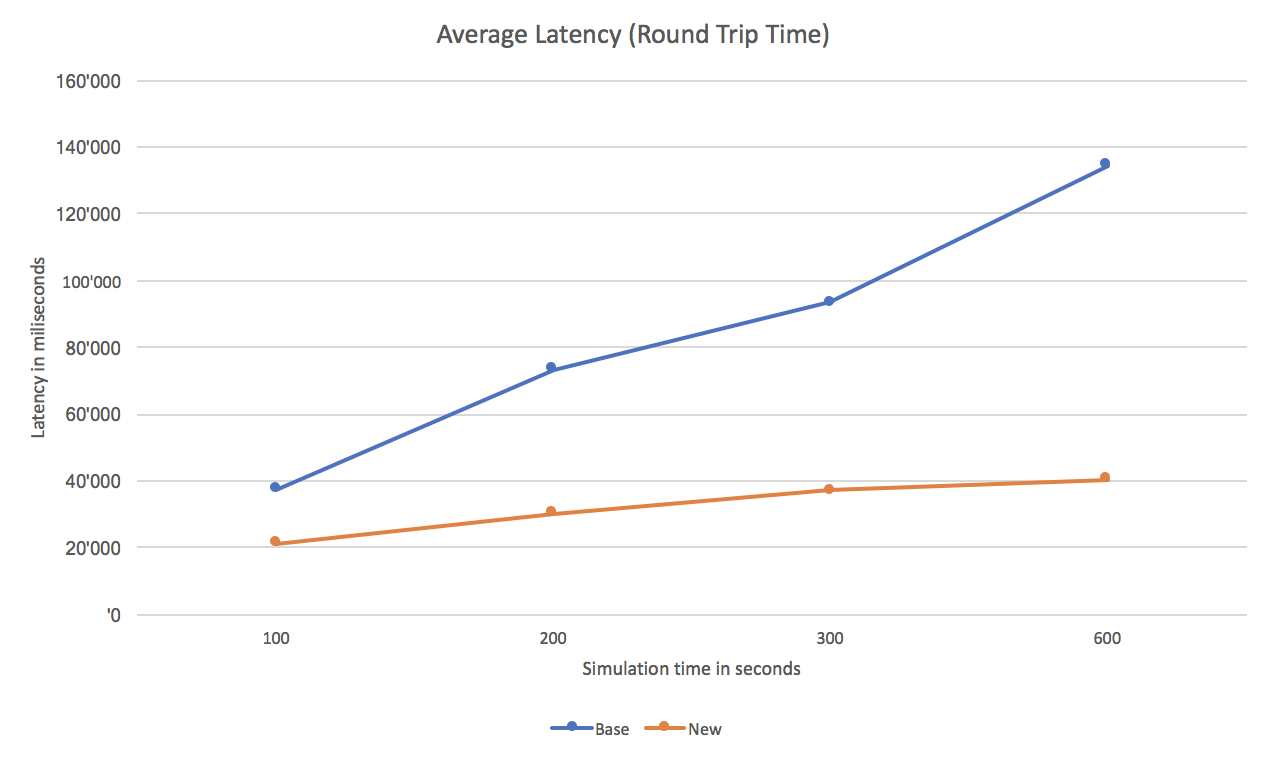
\includegraphics[scale=0.6]{chapter-5/scenario2latency}
  \caption{Latency of both implementations over simulation time}
  \label{fig:scenario2latency}
\end{figure}

\vspace{5mm} %5mm vertical space

In the static and dynamic scenarios, the latency time is around 20 seconds, which is too high for real-time applications. But it can be used well in background processes, like downloading maps, weather forecast or entertainment media.

As an attempt to solve the problem mentioned in figure \ref{fig:scenario2extended}, overhearing of unsolicited data was implemented. Different combinations have been tried with overhearing and dropping of unsolicited data. Overheard data could be used to add new next hops to the FIB entry creating potential routes. These alternative routes, could be used in case the primary route fails at some time. Overhearing data did yield much more next hops within the FIB entry and therefore many distinct routes, but did not result in better performance. Incrementing the cost at every successful transmission led to overheard FIB entries having similar costs like the originally intended routes mixing them up. This also led to worse results and will need further investigation into this topic on how to increment and decrement the cost according to some defined metric, while implementing some kind of mechanism, like an unused cost band, that separates the overheard routes from the originally intended ones.


